\section{Keyframe-Based Image Captioning}

% We also explore a different approach to video captioning, focusing on keyframe-based image captioning. This method leverages the strengths of image captioning models to generate captions for selected keyframes from videos, rather than processing the entire video sequence.

Beyond the primary video-level architecture, we further investigate a complementary paradigm that treats video captioning as a sequence of keyframe-driven image-captioning tasks. In this variant, keyframes are first distilled from the clip and each is captioned by a image-captioning model, rather than processing the entire video sequence. 


\subsection{Keyframe Selection}

The keyframe selection procedure is designed to minimize redundancy and extract only those frames that represent significant visual changes within the video. This process involves the following steps:

\begin{enumerate}[nosep]
    \item Frame Sampling: Frames are initially sampled from the video at a rate of 1 frame per second (fps). This sampling rate substantially reduces the processing load while maintaining a linear runtime relative to the video duration, which is well-suited for short, single-activity videos typical of the MSVD dataset.
    \item Feature Extraction via Visual Embedding: Each sampled frame is transformed into a high-dimensional feature vector using a Vision Transformer (google/vit-base-patch16-224-in21k~\cite{google-vit-base-patch16-224-in21k}) model pre-trained on the ImageNet-21k dataset. ViT embeddings were selected for their demonstrated robustness to common visual artifacts such as motion blur and variations in illumination, rendering them a reliable foundation for change detection.
    \item Similarity-Based Filtering: A frame is designated as a keyframe if its visual representation is sufficiently dissimilar from that of the preceding keyframe. This determination is made using a cosine similarity metric. A frame is added to the keyframe set if the cosine similarity score between its embedding and that of the last accepted keyframe is below a threshold of 0.95.
\end{enumerate}



\subsection{Image Captioning Model}

\subsubsection{Model Architecture}
The image captioning model employs a sophisticated encoder-decoder architecture, integrating a pre-trained Vision Transformer (ViT) as the encoder and a pre-trained Transformer-based language model (T5) as the decoder.

\begin{figure}[H]
  \centering
  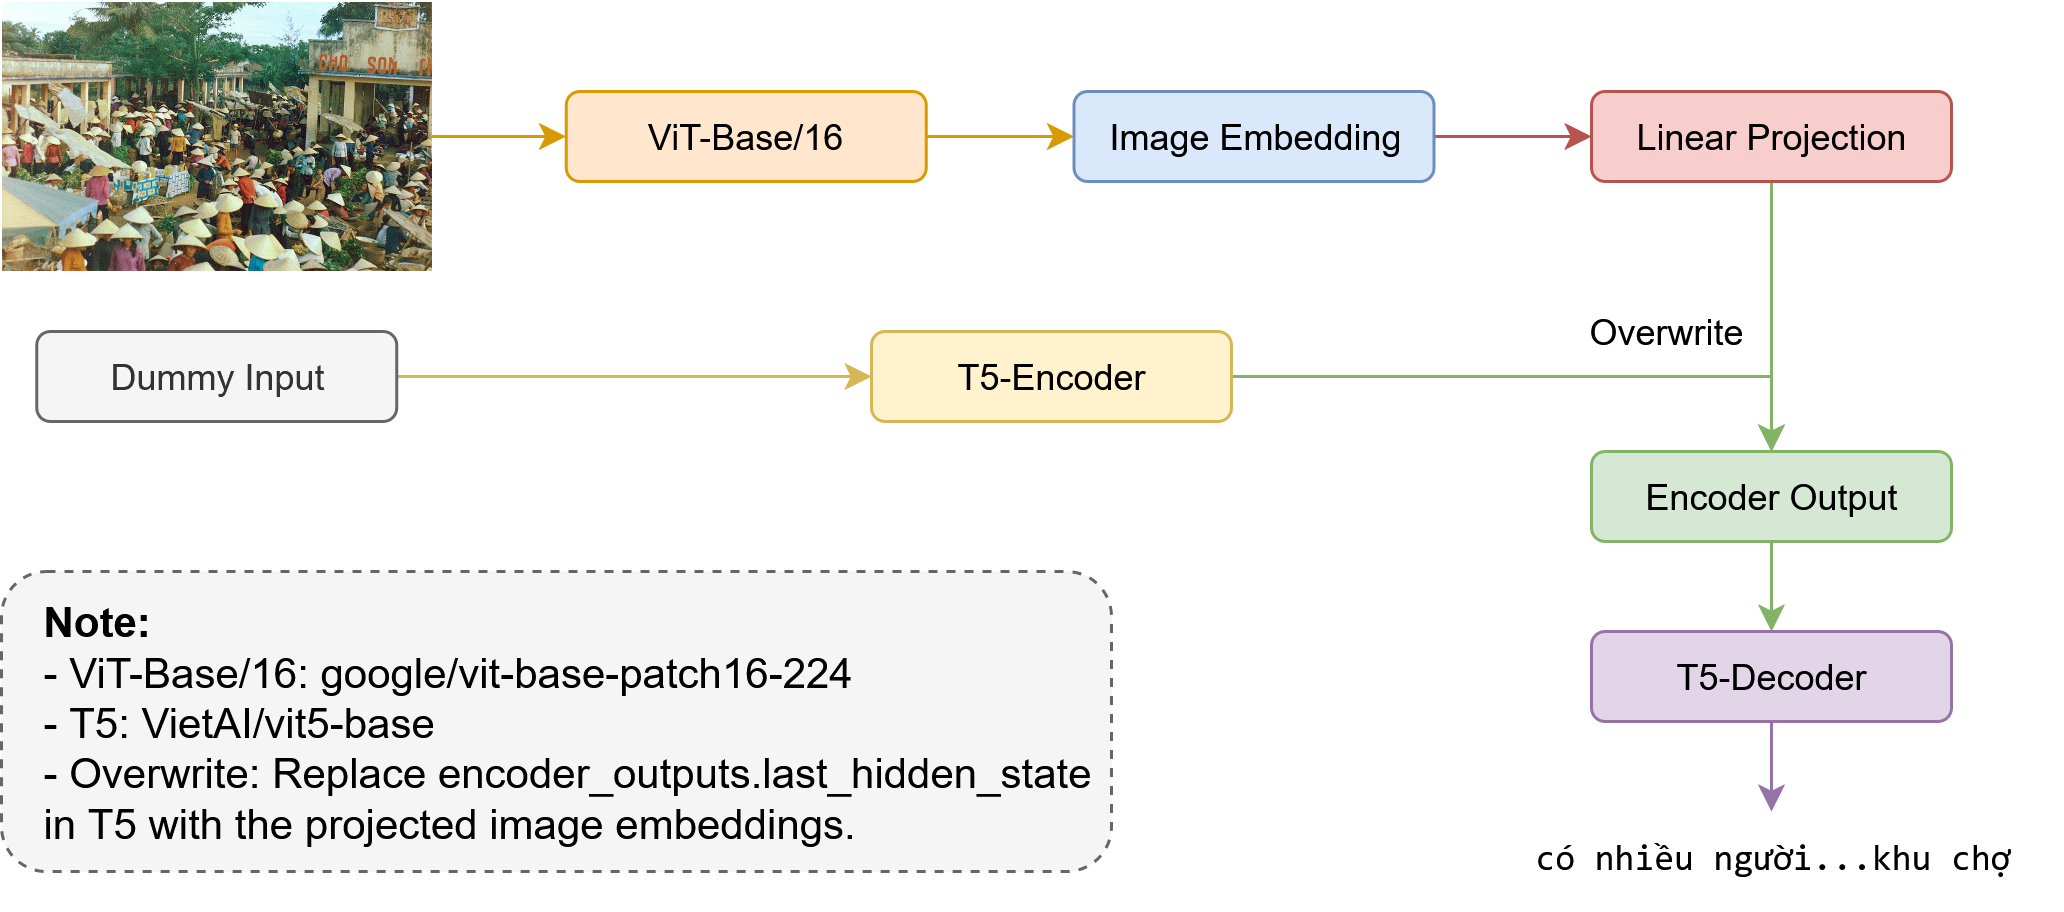
\includegraphics[width=\textwidth]{image/img-captioning-archi.png}
  \caption{The architecture of the ViT-T5 image captioning model, illustrating the integration of the Vision Transformer (ViT) encoder and the T5 decoder.}
  \label{fig:img_cap_archi}
\end{figure}



The visual encoder is a ViT-Base/16~\cite{google-vit-base-patch16-224} model, pre-trained on the ImageNet-21k dataset. Its function is to process an input image and generate a sequence of patch embeddings, which serve as a rich, high-dimensional representation of the image's content.

The text decoder is based on the VietAI/vit5-base~\cite{phan-etal-2022-vit5} model, a T5 variant specifically pre-trained for the Vietnamese language. To bridge the modality gap between the visual encoder and the text decoder, a dedicated interface mechanism was implemented. A linear projection layer maps the embedding dimension of the ViT's output features to the expected hidden dimension ($d_{\text{model}}$) of the T5 decoder.

During the forward pass, the projected visual features directly substitute the output of the T5's own text encoder. Consequently, the T5 decoder's cross-attention mechanism attends directly to this sequence of visual embeddings, enabling it to generate a textual description conditioned on the image content. For generation, the model utilizes a beam search with a beam width of 3 to produce fluent and coherent captions.

\subsubsection{Training Procedure}
The model was trained using a parameter-efficient fine-tuning (PEFT) strategy to leverage the knowledge from the pre-trained components while minimizing computational cost and the risk of catastrophic forgetting. During this phase, the weights of the entire ViT encoder and the T5 text encoder were frozen and did not receive updates. Only the parameters of the T5 decoder, the final language model head, and the intermediary linear projection layer were made trainable.

The model was optimized by minimizing the standard cross-entropy loss between the predicted token sequence and the ground-truth captions. We employed the AdamW optimizer with an initial learning rate of $5 \times 10^{-5}$ and a weight decay of $1 \times 10^{-4}$. The learning rate was dynamically adjusted throughout training using a Cosine Annealing schedule with warm restarts.

Training was conducted for a maximum of 8 epochs. To prevent overfitting and select the best-performing model, an early stopping criterion was implemented. This mechanism monitored the validation loss at the end of each epoch and terminated the training process if no improvement was observed for 5 consecutive epochs. The model checkpoint that achieved the lowest validation loss was saved and used for all subsequent evaluations and inference tasks.

